\chapter{Penrose-Diagramme und die Entstehung eines realen Schwarzen Lochs}

Das Kruskal-Bild liefert eine elegante Beschreibung der Umgebung eines Schwarzschild-Horizonts, doch ein reales Schwarzes Loch ist nicht ewig vorhanden: Es entsteht, wenn Materie kollabiert. Welche Teile des erweiterten Bildes bleiben bei dieser physikalischen Entwicklung erhalten? Um diese Frage zu beantworten, brauchen wir ein Diagramm, das eine ganze Raumzeit umfasst und die Bewegung des Lichts zuverlässig wiedergibt. Zunächst kompaktifizieren wir die flache Raumzeit, dann die Schwarzschild-Raumzeit und fügen schließlich die passenden Teile über eine einfallende Strahlungsschale hinweg zusammen.

\section{In Horizontnähe: Rückblick auf Kruskal und die vier Quadranten}

Wir setzen genau dort an, wo die vorige Vorlesung endete. Sehr nahe am Schwarzschild-Horizont sieht die Geometrie lokal wie flacher Raum aus. Der Horizont selbst verhält sich wie der Ort hyperbolischer Polarkoordinaten, ähnlich wie bei beschleunigten Koordinaten in der gewöhnlichen Minkowski-Raumzeit. In diesem lokalen Bild gilt von Anfang an eine Regel, von der wir nicht abweichen: Radiale Lichtstrahlen werden unter \(45^\circ\) gezeichnet, und jede zeitartige Weltlinie muss steiler verlaufen als diese lichtartigen Linien.

Die Koordinaten in diesem Rückblick stellt man sich am besten als Zeit und Raum vor, wie sie ein frei fallender Beobachter wahrnimmt. In diesen lokal inertialen Koordinaten sieht die Umgebung des Horizonts nahezu flach aus. Ein Beobachter, der außerhalb des Lochs auf einem festen Radius verharrt, ist jedoch nicht inertial. Relativ zum frei fallenden Bezugssystem beschreibt eine solche Person eine beschleunigte Kurve. Je näher man am Horizont verharrt, desto größer muss die Beschleunigung sein, um dort zu bleiben. Darin besteht die physikalische Bedeutung der Familie äußerer Kurven, die rechts an der Tafel eingezeichnet ist.

\begin{figure}[htbp]\centering
\includegraphics[width=0.72\textwidth]{lecture_08_figure_02.png}\caption{Tafelskizze der Geometrie in Horizontnähe mit vier Bereichen. Die roten Kurven im Außenbereich zeigen eine Familie von Weltlinien bei festem Radius, auf denen Beobachter verharren.}\lectureframe{00:02:54}\end{figure}

\begin{figure}[htbp]\centering
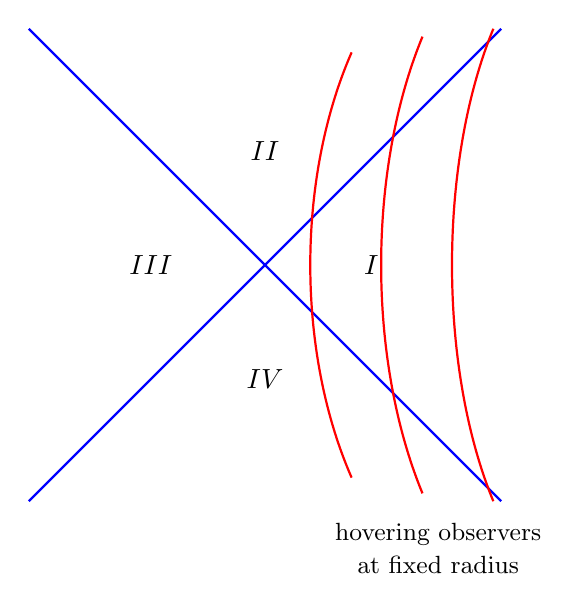
\begin{tikzpicture}[scale=1.0]
\draw[thick,blue] (-3,3) -- (3,-3);
\draw[thick,blue] (-3,-3) -- (3,3);

\draw[red,thick] (1.1,-2.7) .. controls (0.4,-1.1) and (0.4,1.1) .. (1.1,2.7);
\draw[red,thick] (2.0,-2.9) .. controls (1.3,-1.2) and (1.3,1.2) .. (2.0,2.9);
\draw[red,thick] (2.9,-3.0) .. controls (2.2,-1.3) and (2.2,1.3) .. (2.9,3.0);

\node at (1.35,0.0) {$I$};
\node at (0.0,1.45) {$II$};
\node at (-1.45,0.0) {$III$};
\node at (0.0,-1.45) {$IV$};

\node[align=center] at (2.2,-3.6) {\small hovering observers\\\small at fixed radius};
\end{tikzpicture}\caption{Saubere Neuzeichnung der kruskalartigen Kausalstruktur aus dem Rückblick. Bereich \(I\) ist der Außenbereich, Bereich \(II\) das unausweichliche Innere, und die Bereiche \(III\) und \(IV\) gehören zur formalen Erweiterung, die wir später für ein reales, durch Kollaps entstandenes Schwarzes Loch verwerfen.}\end{figure}

Damit lässt sich bereits beschreiben, was ein Schwarzes Loch bewirkt. Im Außenbereich \(I\) können Objekte und Signale nach innen gelangen, aber auch draußen bleiben oder wieder nach außen zurückkehren. In Bereich \(II\) hingegen steht das Kausalurteil fest. Wer sich einmal im Inneren befindet, kann auf keinem zukünftigen kausalen Weg mehr in den Außenbereich zurückgelangen. Um aus Bereich \(II\) in einen der beiden Außenbereiche zu entkommen, müsste die Weltlinie irgendwo flacher als \(45^\circ\) verlaufen und wäre damit schneller als das Licht. Jede zulässige zukünftige zeitartige Weltlinie endet an der Singularität.

Dieser einleitende Rückblick ist nicht bloß eine Wiederholung. Er bereitet das Hauptthema des Kapitels vor. Das Kruskal-Bild ist nützlich, doch für ein reales Schwarzes Loch ist nicht jeder Teil davon physikalisch relevant.

\begin{classroomqa}\audiencequestion{Was sind die Achsen des Diagramms, und zu welchen Beobachtern gehören die Weltlinien bei fester Position, die rot eingezeichnet sind?}\lecturerresponse{Die Achsen stellen Zeit und Raum in Koordinaten dar, die für einen frei fallenden Beobachter natürlich sind. In Horizontnähe sieht dieser Beobachter eine nahezu gewöhnliche flache Raumzeit. Die roten Kurven bei konstanter Position gehören dagegen zu Beobachtern, die außerhalb des Lochs stationär gehalten werden. Ihre Weltlinien sind beschleunigt; die erforderliche Beschleunigung nimmt zum Horizont hin zu.\lecturetimestamp{00:05:58--00:06:47}}\end{classroomqa}

\section{Warum kompaktifizieren? Von der unendlichen Raumzeit zur endlichen Tafel}

Der nächste Schritt ist methodischer Art. Die Nullrichtungen der Diagramme reichen bis ins Unendliche, und auch die Zeit selbst ist unendlich. Daher können wir die ganze Raumzeit nicht auf einer gewöhnlichen Tafel darstellen, solange wir die Koordinaten nicht ändern. Die Motivation des Dozenten ist ganz konkret: Wenn wir alles auf einmal sehen und die globale Kausalstruktur untersuchen wollen, brauchen wir ein Verfahren, das eine unendliche Raumzeit in einen endlichen Bereich abbildet und dabei die Lichtstrahlen erkennbar lässt.

Daher geht er zunächst zum einfachen Fall zurück, zur guten alten flachen Raumzeit. Da die Probleme, die uns interessieren, kugelsymmetrisch sind, lassen wir die Winkelrichtungen weg und behalten nur die Zeit und die radiale Koordinate bei. Wir verwenden die Koordinaten \(T\) und \(R\) mit
\[
R\ge 0,
\]
da ein negativer radialer Abstand in Polarkoordinaten keine Bedeutung hat. Außerdem wählen wir Einheiten, in denen
\[
c=1.
\]
Mit dieser Konvention werden radiale Nullbewegungen unter \(45^\circ\) gezeichnet.

Bevor wir die kompaktifizierende Abbildung einführen, nimmt sich die Vorlesung etwas Zeit, um uns im \(T\)-\(R\)-Diagramm zu orientieren. Man zeichnet die Zeitachse, die radiale Achse, einige Schnitte konstanter Zeit \(T=0,\pm1,\pm2\) und einige Linien konstanten Radius \(R=1,2,3\). Das ist keine leere Formalität. Es liefert Orientierungspunkte und macht deutlich, welche Eigenschaften erhalten bleiben sollen, wenn wir das Diagramm später auf endliche Größe zusammendrücken.

Auch der Ursprung birgt einen subtilen, aber wichtigen didaktischen Punkt. Im reduzierten radialen Bild scheint ein genau auf \(R=0\) gerichteter Lichtstrahl am Ursprung abzuprallen und wieder nach außen zurückzukehren. Doch physikalisch wird nichts an einer Wand reflektiert. In der vollständigen kugelsymmetrischen Geometrie durchquert der Strahl einfach den Ursprung und tritt auf der anderen Seite wieder aus. Der scheinbare Abprall ergibt sich allein daraus, dass wir die Halbebene \(R\ge 0\) betrachten.

Ebenso sieht ein Lichtstrahl, der am Ursprung vorbeigeht, zunächst fast genauso aus: Er erreicht den Punkt der größten Annäherung und wendet sich dann wieder nach außen. In diesen Koordinaten kann es sogar so aussehen, als hätte ihn etwas vom Ursprung abgestoßen. Doch auch das ist lediglich eine koordinatenabhängige Beschreibung der vertrauten Drehimpulsbarriere und keine neue Kraft. Der Dozent verweilt bei diesen Beispielen, weil das Publikum dem Diagramm vertrauen soll, bevor er es verformt.

Nun kommt der entscheidende Schritt. Wir werden das Bild stauchen und strecken, aber eines bleibt unverändert: Radiale Lichtstrahlen müssen weiterhin unter \(45^\circ\) verlaufen. Genau darum geht es bei der Kompaktifizierung.

\begin{classroomqa}\audiencequestion{Gibt es am gewählten Ursprung etwas physikalisch Besonderes, und sind die scheinbar gekrümmten Strahlen ein Hinweis auf eine dort wirkende Kraft?}\lecturerresponse{Nein. In diesem Stadium ist der Ursprung lediglich das Zentrum, das durch die Kugelkoordinaten festgelegt wird. Der scheinbare Abprall und die Krümmung entstehen dadurch, dass die vollständige räumliche Bewegung auf \(R\geq0\) reduziert wird. Eine Symmetrie kann ein Zentrum nützlich machen, wie beim Sonnensystem, doch die Wahl der Koordinaten platziert dort weder ein Schwarzes Loch noch eine reflektierende Wand.\lecturetimestamp{00:16:27--00:17:08}}\end{classroomqa}

\section{Flache Raumzeit in Nullkoordinaten und Penrose-Form}

Um die Verformung präzise zu beschreiben, führen wir Nullkoordinaten ein. Dies ist der mathematisch klare Teil der Vorlesung, und an der Tafel wird der Schritt ausdrücklich ausgeführt.

\begin{figure}[htbp]\centering
\includegraphics[width=0.82\textwidth]{lecture_08_figure_03.png}\caption{Die freie \(T\)-\(R\)-Tafel bei der Einführung von \(T^+=T+R\) und \(T^-=T-R\). Der reduzierte radiale Ursprung ist die blaue vertikale Linie \(R=0\).}\lectureframe{00:19:45}\end{figure}

Wir definieren
\begin{align}
T^+ &= T+R, \\
T^- &= T-R.
\end{align}
Diese Koordinaten sind an radiale Nullbewegungen angepasst. Für einen einlaufenden radialen Lichtstrahl gilt \(T^+=\text{const}\), für einen auslaufenden radialen Lichtstrahl dagegen \(T^-=\text{const}\).

\paragraph{Herleitung.}
Die Linie \(R=0\) nimmt in diesen Koordinaten eine besonders einfache Form an. Tatsächlich gilt
\begin{align}
R=0
&\iff T+R=T-R \\
&\iff T^+=T^-.
\end{align}
Die gesamte zeitartige Randlinie \(R=0\) wird also durch die einzige Beziehung
\begin{equation}
R=0 \iff T^+=T^-.
\end{equation}beschrieben.

\begin{figure}[htbp]\centering
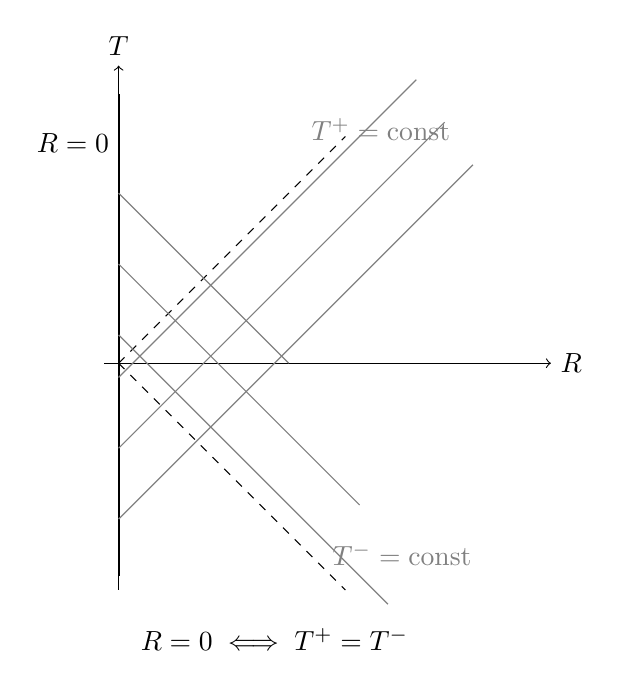
\begin{tikzpicture}[scale=0.9]
\draw[->] (-0.2,0) -- (6.1,0) node[right] {$R$};
\draw[->] (0,-3.2) -- (0,4.2) node[above] {$T$};

\draw[thick] (0,-3.0) -- (0,3.8);
\node[left] at (0,3.1) {$R=0$};

\draw[dashed] (0,0) -- (3.2,3.2);
\draw[dashed] (0,0) -- (3.2,-3.2);

\draw[gray] (0,2.4) -- (2.4,0);
\draw[gray] (0,1.4) -- (3.4,-2.0);
\draw[gray] (0,0.4) -- (3.8,-3.4);

\draw[gray] (0,-2.2) -- (5.0,2.8);
\draw[gray] (0,-1.2) -- (4.6,3.4);
\draw[gray] (0,-0.2) -- (4.2,4.0);

\node[gray] at (3.7,3.3) {$T^+=\mathrm{const}$};
\node[gray] at (4.0,-2.7) {$T^-=\mathrm{const}$};

\node at (2.2,-3.9) {$R=0 \iff T^+=T^-$};
\end{tikzpicture}\caption{Eine saubere Neuzeichnung im \(T\)-\(R\)-Diagramm. Die beiden Nullstrahlfamilien sind die Niveaumengen von \(T^+\) und \(T^-\), und die Linie \(R=0\) ist gleichbedeutend mit \(T^+=T^-\).}\end{figure}

Nun kompaktifizieren wir. Wir führen zwei neue Nullkoordinaten \(U^\pm\) ein, die jeweils aus der entsprechenden Koordinate \(T^\pm\) mit derselben beschränkten monotonen Funktion \(F\) gewonnen werden:
\begin{align}
U^+ &= F(T^+), &
U^- &= F(T^-),
\end{align}
Dabei gilt
\begin{equation}
F(+\infty)=1,
\qquad
F(-\infty)=-1.
\end{equation}
Die in der Vorlesung verwendete praktische Wahl lautet
\begin{equation}
F(x)=\tanh x,
\end{equation}
sodass
\begin{equation}
U^+ = \tanh(T^+),
\qquad
U^- = \tanh(T^-).
\end{equation}
gilt. Der Tangens hyperbolicus ist nichts Besonderes. Er ist einfach eine glatte Funktion mit dem passenden Grenzverhalten und bildet deshalb unendliche Koordinatenbereiche auf endliche ab.

Die Nullstruktur bleibt aus einem einfachen Grund erhalten. Gilt für einen einlaufenden radialen Lichtstrahl \(T^+=\text{const}\), so gilt
\[
U^+=F(T^+)=\text{const},
\]
und ebenso gilt für einen auslaufenden radialen Lichtstrahl mit \(T^-=\text{const}\)
\[
U^-=F(T^-)=\text{const}.
\]
Die Kompaktifizierung parametrisiert also die beiden Nullrichtungen getrennt neu, sodass radiale Lichtstrahlen weiterhin unter \(45^\circ\) verlaufen. Auch die Ursprungslinie wird auf ebenso einfache Weise abgebildet:
\[
T^+=T^- \Longrightarrow U^+=U^-.
\]

Damit ist die unendliche Halbebene der flachen Raumzeit auf ein endliches Dreieck zusammengedrückt. Anschließend zeigt die Vorlesung, wie dessen Ränder zu lesen sind. Die räumliche Unendlichkeit schrumpft zu einem einzigen Punkt \(i^0\) zusammen. Die zukünftige und die vergangene zeitartige Unendlichkeit sind \(i^+\) und \(i^-\). Die beiden lichtartigen Ränder sind \(\mathcal{I}^+\) und \(\mathcal{I}^-\), oft „Scri-plus“ und „Scri-minus“ ausgesprochen: Dort beginnen beziehungsweise enden einlaufende und auslaufende Lichtstrahlen.

\begin{figure}[htbp]\centering
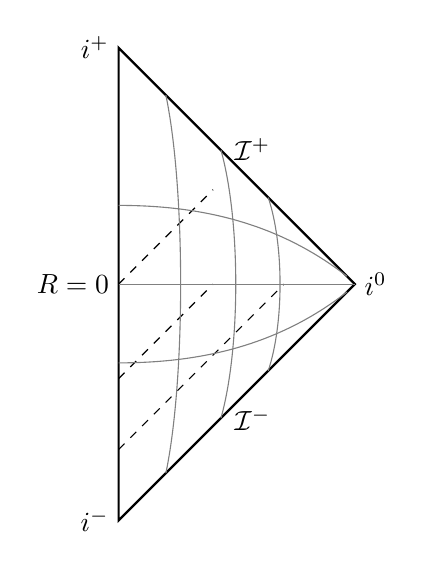
\begin{tikzpicture}[scale=1.0]
\draw[thick] (0,-3) -- (0,3) -- (3,0) -- cycle;

\node[left] at (0,3) {$i^+$};
\node[left] at (0,-3) {$i^-$};
\node[right] at (3,0) {$i^0$};
\node[left] at (0,0) {$R=0$};
\node[above right] at (1.35,1.45) {$\mathcal{I}^+$};
\node[below right] at (1.35,-1.45) {$\mathcal{I}^-$};

\draw[dashed] (0,-2.1) -- (2.1,0.0);
\draw[dashed] (0,-1.2) -- (1.2,0.0);
\draw[dashed] (0,0.0) -- (1.2,1.2);

\draw[gray] (0,0) -- (3,0);
\draw[gray] (0,1.0) .. controls (1.0,1.0) and (2.0,0.8) .. (2.9,0.1);
\draw[gray] (0,-1.0) .. controls (1.0,-1.0) and (2.0,-0.8) .. (2.9,-0.1);

\draw[gray] (0.6,-2.4) .. controls (0.85,-1.2) and (0.85,1.2) .. (0.6,2.4);
\draw[gray] (1.3,-1.7) .. controls (1.55,-0.8) and (1.55,0.8) .. (1.3,1.7);
\draw[gray] (1.9,-1.1) .. controls (2.1,-0.5) and (2.1,0.5) .. (1.9,1.1);
\end{tikzpicture}\caption{Penrose-Diagramm der radial reduzierten flachen Raumzeit. Kurven konstanter Zeit verlaufen nach außen in Richtung \(i^0\), während Kurven konstanten Radius von \(i^-\) in Richtung \(i^+\) aufsteigen.}\end{figure}

Ein letzter Punkt aus der Vorlesung sollte im Gedächtnis bleiben. Diese Diagramme erhalten \emph{nicht} die metrischen Abstände. Sie erhalten die Kausalstruktur. Darauf kommt es uns an.

\begin{classroomqa}\audiencequestion{Sollen die kompaktifizierten Linien konstanter Zeit gerade verlaufen?}\lecturerresponse{Nur der symmetrische Schnitt \(T=0\) ist für die gewählte Abbildung gerade. Die übrigen Kurven mit konstantem \(T\) sind gekrümmt; ihre genaue Form hängt von der kompaktifizierenden Funktion ab. Sehr späte Schnitte rücken immer näher an den oberen Rand, obwohl die gewöhnliche Zeit unbegrenzt weiterläuft.\lecturetimestamp{00:29:11--00:30:12}}\end{classroomqa}

\section{Die kompaktifizierte Schwarzschild-Geometrie}

Mit der Konstruktion für den flachen Raum als Grundlage kehren wir nun zum Schwarzen Loch zurück und gehen genauso vor. Wir kompaktifizieren die Kruskal-Geometrie, indem wir Nullkoordinaten einführen und die unendlichen Bereiche auf eine endliche Figur zusammendrücken. Der Dozent beschreibt das Ergebnis als schräges Rechteck oder rautenförmiges Kausaldiagramm: Der Horizont erscheint als lichtartiger Rand, die Weltlinien der schwebenden Beobachter im Außenbereich bleiben außerhalb davon, und der Innenbereich endet an einer Singularität, die nun auf der Seite sichtbar ist.

Der entscheidende physikalische Punkt ist, dass die Singularität für einen frei fallenden Beobachter \emph{nicht} in unendlicher Ferne liegt. Nach dem Überschreiten des Horizonts bleibt bis zum Aufprall auf die Singularität nur eine endliche Eigenzeit. Das Penrose-Diagramm macht dies unausweichlich sichtbar.

Der Horizont wird erneut durch die Schwarzschild-Bedingung bestimmt:
\begin{equation}
1-\frac{2MG}{r}=0
\qquad \Longleftrightarrow \qquad
r=2MG.
\end{equation}
Die Gleichheit \(r=2MG\) kennzeichnet den Radius, an dem der Schwarzschild-Faktor sein Vorzeichen wechselt.

\begin{figure}[htbp]\centering
\includegraphics[width=0.72\textwidth]{lecture_08_figure_04.png}\caption{Tafelskizze, die das formale erweiterte Bild dem physikalisch relevanten Bereich des Schwarzen Lochs gegenüberstellt. Die rote Beschriftung \emph{Singularität} ist an der Tafel ausdrücklich eingezeichnet.}\lectureframe{00:37:59}\end{figure}

\begin{figure}[htbp]\centering
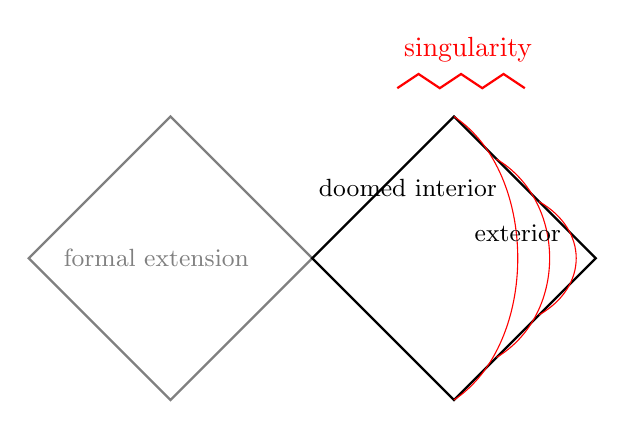
\begin{tikzpicture}[scale=0.9]
\draw[gray,thick] (-4,0) -- (-2,2) -- (0,0) -- (-2,-2) -- cycle;
\draw[thick] (0,0) -- (2,2) -- (4,0) -- (2,-2) -- cycle;

\draw[red,thick] (1.2,2.4) -- (1.5,2.6) -- (1.8,2.4) -- (2.1,2.6) -- (2.4,2.4) -- (2.7,2.6) -- (3.0,2.4);
\node[red] at (2.2,2.95) {singularity};

\draw[red] (2.0,-2.0) .. controls (3.2,-1.2) and (3.2,1.2) .. (2.0,2.0);
\draw[red] (2.6,-1.4) .. controls (3.6,-0.8) and (3.6,0.8) .. (2.6,1.4);
\draw[red] (3.2,-0.8) .. controls (3.9,-0.4) and (3.9,0.4) .. (3.2,0.8);

\node at (2.9,0.35) {\small exterior};
\node at (1.35,1.0) {\small doomed interior};
\node[gray] at (-2.2,0.0) {\small formal extension};
\end{tikzpicture}\caption{Eine zurückhaltende Neuzeichnung der in der Vorlesung hervorgehobenen Kausalstruktur: der erhaltene Außenbereich, das unausweichliche Innere, die zukünftige Singularität und der Kontrast zum zusätzlichen formalen Teil der Erweiterung.}\end{figure}

Die Vorlesung ist hier sehr direkt. Befindet man sich im Außenbereich, kann man noch entkommen oder hineinfallen. Befindet man sich im Inneren, ist man verloren. Das Diagramm sagt bereits alles Wesentliche über zukünftige kausale Bewegung aus.

Die Quadranten \(III\) und \(IV\) sind legitime Teile der maximal erweiterten Kruskal-Lösung. Bereich \(III\) stellt einen zweiten Außenbereich dar, und Bereich \(IV\) ist der zeitumgekehrte Bereich des Schwarzen Lochs. In der Raumzeit eines gewöhnlichen, durch Kollaps entstandenen Schwarzen Lochs treten sie jedoch nicht auf. Die erweiterte Lösung ist mathematisch gerade deshalb lehrreich, weil die Konstruktion des Kollapses zeigen wird, welche Teile verworfen werden müssen.

\section{Räumliche Schnitte, Zweisphären und die Einstein--Rosen-Brücke}

Betrachten wir nun einen räumartigen Schnitt im kompaktifizierten Diagramm und fragen, wie dieser Schnitt als \emph{Raum} statt als Raumzeit aussieht. Hier kommt das Wurmlochbild ins Spiel; dabei darf das räumliche Bild dem Kausalargument nicht vorauseilen.

Da die Winkelrichtungen unterdrückt wurden, steht jeder Punkt des radialen Diagramms für eine Zweisphäre. Bei Schwarzschild-Radius \(r\) beträgt ihre Fläche
\begin{equation}
A=4\pi r^2.
\end{equation}
Ein räumartiger Schnitt besteht daher aus einer Familie von Zweisphären, nicht bloß aus einer eindimensionalen Kurve. Ihre Größe ändert sich, wenn man sich entlang des Schnitts bewegt.

In großer Entfernung sind die Sphären sehr groß. Bewegt man sich nach innen, nimmt ihr Radius ab, bis er am Horizont einen Minimalwert erreicht:
\begin{equation}
r_{\min}=2MG.
\end{equation}
Geht man durch die formale Erweiterung weiter, werden die Sphären zu einer weiteren asymptotischen Seite hin wieder größer. Das ist das Bild der Einstein--Rosen-Brücke.

\begin{figure}[htbp]\centering
\includegraphics[width=0.72\textwidth]{lecture_08_figure_05.png}\caption{Das erweiterte Kruskal-Diagramm mit dem grünen räumartigen Schnitt, aus dem die Brückengeometrie konstruiert wird. Jeder Punkt auf diesem Schnitt steht für eine Zweisphäre; ihr minimaler Radius ist mit \(r=2MG\) markiert.}\lectureframe{00:41:30}\end{figure}

An der Tafel ist nur ein Teil des betreffenden Schwarzschild-Faktors dargestellt,
\begin{equation}
1-\frac{2MG}{r},
\end{equation}
und der Hals liegt beim selben besonderen Radius \(r=2MG\).

\begin{figure}[htbp]\centering
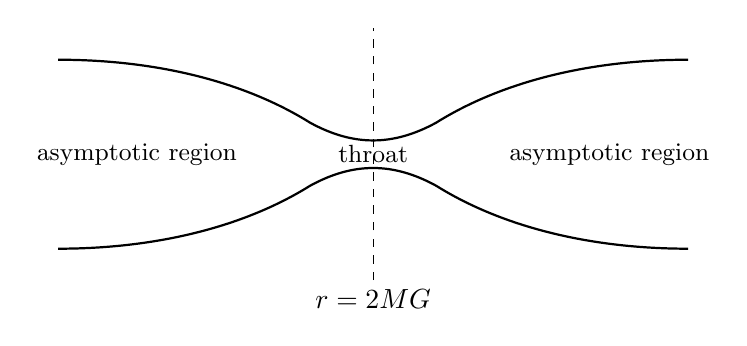
\begin{tikzpicture}[scale=1.0]
\draw[thick] (-4,1.2)
.. controls (-2.7,1.2) and (-1.6,0.9) .. (-0.8,0.4)
.. controls (-0.25,0.1) and (0.25,0.1) .. (0.8,0.4)
.. controls (1.6,0.9) and (2.7,1.2) .. (4,1.2);

\draw[thick] (-4,-1.2)
.. controls (-2.7,-1.2) and (-1.6,-0.9) .. (-0.8,-0.4)
.. controls (-0.25,-0.1) and (0.25,-0.1) .. (0.8,-0.4)
.. controls (1.6,-0.9) and (2.7,-1.2) .. (4,-1.2);

\draw[dashed] (0,-1.6) -- (0,1.6);
\node[below] at (0,-1.6) {$r=2MG$};
\node at (0,0) {\small throat};
\node at (-3.0,0) {\small asymptotic region};
\node at (3.0,0) {\small asymptotic region};
\end{tikzpicture}\caption{Schematischer räumlicher Schnitt durch die erweiterte Schwarzschild-Geometrie. Dies ist eine vorsichtige Rekonstruktion des Brückenbilds aus der Vorlesung, keine tatsächliche Einbettungsrechnung.}\end{figure}

Nun folgt die Korrektur. Der Schnitt legt eine Brücke zwischen zwei asymptotischen Bereichen nahe und damit den Gedanken, man könne durch den Hals von einem Universum ins andere reisen. Die Vorlesung lässt diesen Eindruck zunächst entstehen und widerlegt ihn dann mithilfe der Kausalstruktur. Um von einem Außenbereich zum anderen zu gelangen, müsste eine Weltlinie im Penrose-Diagramm irgendwo flacher als eine Nullinie unter \(45^\circ\) verlaufen. Das ist verboten. Die Einstein--Rosen-Brücke ist also nicht durchquerbar.

Der Dozent betont auch, warum das räumliche Bild irreführend sein kann. Es zeigt \emph{den Raum zu einem Zeitpunkt}; doch es steht schlicht nicht genug Kausalzeit zur Verfügung, um hindurchzugelangen. Vereinfacht gesagt öffnet und schließt sich die Brücke, bevor irgendetwas sie durchqueren kann. Noch besser: Man schaut einfach wieder auf das Penrose-Diagramm und liest die kausale Antwort ab.

\section{Ein reales Schwarzes Loch aus einer einfallenden lichtartigen Schale bilden}

An diesem Punkt wechselt die Vorlesung vollständig das Problem. Wir lesen nicht länger die Eigenschaften eines ewigen Schwarzen Lochs ab, sondern konstruieren ein reales.

Das Modell ist der Einfachheit halber gewählt. Wir stellen uns keinen kollabierenden Stern mit komplizierter innerer Struktur vor, sondern eine dünne kugelförmige Schale einfallender Strahlung. Sie besteht aus Licht und bewegt sich daher mit Lichtgeschwindigkeit nach innen. Bei hinreichend kleinem Radius ist die Energie in der Schale so stark konzentriert, dass ein Schwarzes Loch entsteht.

Die zweite Zutat ist der Schalensatz in seiner allgemein-relativistischen Form.

\paragraph{Bemerkung.} Bei der in dieser Vorlesung verwendeten kugelsymmetrischen Schale ist der Innenbereich flache Raumzeit, während der Außenbereich Schwarzschild-Geometrie ist. Dies ist der operative Schalensatz beziehungsweise eine Aussage vom Birkhoff-Typ, die in der Vorlesung verwendet wird. Hier wird sie nicht bewiesen.

Der Dozent motiviert dies, indem er zunächst an den Newtonschen Schalensatz erinnert: Innerhalb einer Kugelschale gibt es kein Gravitationsfeld; außerhalb ist das Feld dasselbe wie das einer Punktmasse im Zentrum. Dann formuliert er die entsprechende relativistische Version in der hier benötigten Form: innen ist die Raumzeit flach, außen Schwarzschild. Die Schale kann sich bewegen; die Regel bleibt dieselbe.

Das genügt, um die Kollapsraumzeit zu konstruieren. Die Schale selbst ist lichtartig und muss deshalb unter \(45^\circ\) verlaufen. Auf der einen Seite dieser Nullinie ist die Geometrie flach, auf der anderen Schwarzschild. Die Regel lässt sich so zusammenfassen:
\begin{equation}
\begin{aligned}
\text{inside shell} &= \text{flat spacetime},\\
\text{outside shell} &= \text{Schwarzschild geometry}.
\end{aligned}
\end{equation}

Die Vorschrift zum Zusammenfügen ist dann denkbar einfach:

\begin{enumerate}\item Zeichne das flache Penrose-Diagramm und behalte nur den Bereich innerhalb der einlaufenden Schale.
\item Zeichne das Schwarzschild-Penrose-Diagramm und behalte nur den Bereich außerhalb derselben Schale.
\item Verwirf die falschen Teile.
\item Füge die beiden verbleibenden Teile entlang der Bahn der Schale zusammen.
\end{enumerate}

Genau so geht der Dozent an der Tafel vor: Er verwirft die falsche Hälfte des einen Bildes, verwirft die falsche Hälfte des anderen und fügt die richtigen Hälften entlang der Schale zusammen.

\begin{figure}[htbp]\centering
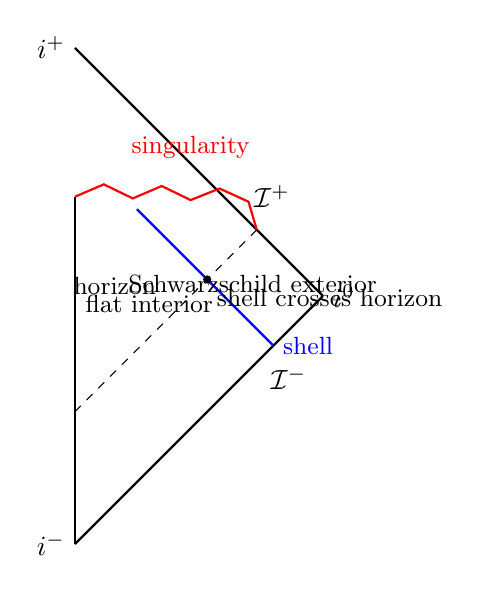
\begin{tikzpicture}[scale=1.05]
\coordinate (im) at (0,-3.0);
\coordinate (ip) at (0,3.0);
\coordinate (i0) at (3.0,0.0);
\coordinate (S)  at (0,1.2);
\coordinate (E)  at (2.2,0.8);
\coordinate (P)  at (2.4,-0.6);
\coordinate (Q)  at (0.75,1.05);
\coordinate (H)  at (0,-1.4);
\coordinate (X)  at (1.6,0.2);

\draw[thick] (im) -- (S);
\draw[thick] (im) -- (i0);
\draw[thick] (ip) -- (i0);

\draw[red,thick] (S) -- (0.35,1.35) -- (0.7,1.18) -- (1.05,1.33) -- (1.4,1.16) -- (1.75,1.30) -- (2.1,1.14) -- (E);
\node[red,above] at (1.4,1.55) {\small singularity};

\draw[thick,blue] (P) -- (Q);
\node[blue,right] at (P) {\small shell};

\draw[dashed] (H) -- (E);
\node[above left] at (1.1,-0.1) {\small horizon};

\filldraw (X) circle (1.2pt);
\node[below right] at (X) {\small shell crosses horizon};

\node at (0.9,-0.1) {\small flat interior};
\node at (2.15,0.15) {\small Schwarzschild exterior};

\node[left] at (im) {$i^-$};
\node[left] at (ip) {$i^+$};
\node[right] at (i0) {$i^0$};
\node[below right] at (2.25,-0.75) {$\mathcal{I}^-$};
\node[above right] at (2.05,0.95) {$\mathcal{I}^+$};
\end{tikzpicture}\caption{Kausale Rekonstruktion der Kollapsgeometrie. Die Schale ist eine einlaufende Nullinie; auf ihrer Innenseite bleibt die Raumzeit flach, auf ihrer Außenseite gilt die Schwarzschild-Geometrie.}\end{figure}

\begin{figure}[htbp]\centering
\includegraphics[width=0.76\textwidth]{lecture_08_figure_06.png}\caption{Die fertige Tafelkonstruktion, nachdem der flache Innenbereich und der Schwarzschild-Außenbereich entlang der blauen einfallenden Schale zusammengefügt wurden. Die gestrichelte Linie \(45^\circ\) wird vom zukünftigen Endpunkt der Singularität rückwärts verfolgt, um den Ereignishorizont zu bestimmen.}\lectureframe{00:57:30}\end{figure}

Für die Schale selbst geschieht nichts Besonderes, wenn sie lediglich vom flachen Teil des Diagramms in den Schwarzschild-Teil übergeht. Sie ist eine lichtartige Schale und bewegt sich weiter nach innen, bis sie die Singularität erreicht. Die wesentliche Struktur entsteht nicht durch ein lokales dramatisches Ereignis an der Schale, sondern durch die kausale Ordnung der zusammengefügten Raumzeit.

\begin{classroomqa}\audiencequestion{Gibt es eine Diskontinuität, wenn die kollabierende Schale ihren Schwarzschild-Radius überschreitet?}\lecturerresponse{Nein. Bei diesem Übergang geschieht lokal nichts Singularitätsartiges. Die Schale setzt ihre Nullbahn fort. Das besondere Ereignis ist kausaler Art: Nachdem die Schale ihren eigenen Radius \(2MG\) überschritten hat, kann kein zukünftiger Weg sie mehr ins Unendliche zurückbringen.\lecturetimestamp{00:56:19--00:56:42}}\end{classroomqa}

\section{Der Horizont vor dem Eintreffen: das Rätsel des Ereignishorizonts}

Nun folgt der begriffliche Höhepunkt der Vorlesung. Nachdem die Kollapsraumzeit konstruiert ist, stellt sich ganz natürlich die Frage: Wo liegt der Horizont? Oder, wie der Dozent es formuliert: Wo ist der Punkt, von dem es kein Zurück gibt?

\paragraph{Definition.} Der Ereignishorizont ist die Grenze zwischen Ereignissen, von denen noch ein zukünftiges kausales Signal nach \(\mathcal{I}^+\) gesendet werden kann, und solchen, von denen das nicht möglich ist.

Die Vorlesung bestimmt ihn im Diagramm. Man beginnt an der Ecke, an der die Singularität die zukünftige Nullunendlichkeit trifft, und verfolgt eine Nullinie unter \(45^\circ\) rückwärts. Diese rückwärts verfolgte Nullinie ist der Ereignishorizont.

Dann besteht der Dozent auf einem zweiten Punkt, der den Studierenden Unbehagen bereitet. Der Horizont entsteht nicht erst in dem Augenblick, in dem die Schale ihren eigenen Schwarzschild-Radius überschreitet, und bleibt dann dort. In der vergrößerten Tafelskizze beginnt der Horizont als winziger eingeschlossener Bereich nahe dem Zentrum, breitet sich durch einen Teil der Raumzeit aus, der noch flach ist, und trifft erst später auf die einlaufende Schale. Bei diesem Zusammentreffen überschreitet die Schale ihren eigenen Schwarzschild-Radius. Oberhalb dieses Ereignisses ist der Horizont der gewöhnliche Horizont konstanten Radius des fertig ausgebildeten Schwarzen Lochs.

\begin{figure}[htbp]\centering
\resizebox{0.96\linewidth}{!}{%
\begin{tikzpicture}[scale=1.08,>=Latex]
\coordinate (im) at (0,-3.0);
\coordinate (ip) at (0,3.0);
\coordinate (i0) at (3.0,0.0);
\coordinate (S)  at (0,1.2);
\coordinate (E)  at (2.2,0.8);
\coordinate (P)  at (2.4,-0.6);
\coordinate (Q)  at (0.75,1.05);
\coordinate (H)  at (0,-1.4);
\coordinate (X)  at (1.6,0.2);

\draw[thick] (im) -- (S);
\draw[thick] (im) -- (i0);
\draw[thick] (ip) -- (i0);

\draw[red,thick] (S) -- (0.35,1.35) -- (0.7,1.18) -- (1.05,1.33) -- (1.4,1.16) -- (1.75,1.30) -- (2.1,1.14) -- (E);
\node[red,above left] at (S) {\small singularity};

\draw[very thick,red] (H) -- (E);

\draw[thick,blue] (P) -- (Q);

\filldraw (X) circle (1.2pt);

\draw[gray] (0.0,-2.1) .. controls (0.85,-1.95) and (1.9,-1.3) .. (2.8,-0.2);
\draw[gray] (0.0,-1.2) .. controls (0.95,-1.0) and (1.8,-0.45) .. (2.45,0.35);
\draw[gray] (0.0,-0.2) .. controls (0.8,-0.05) and (1.45,0.35) .. (1.95,0.95);

\node[below right] at (2.28,-0.72) {$\mathcal{I}^-$};
\node[above right] at (2.12,0.92) {$\mathcal{I}^+$};

\draw[very thick,red] (3.2,-1.15) -- (3.75,-1.15);
\node[anchor=west] at (3.85,-1.15) {\small event horizon};
\draw[thick,blue] (3.2,-1.55) -- (3.75,-1.55);
\node[anchor=west] at (3.85,-1.55) {\small infalling shell};
\filldraw (3.48,-1.95) circle (1.2pt);
\node[anchor=west] at (3.85,-1.95)
  {\small shell reaches \(r=2MG\)};
\end{tikzpicture}}\caption{Kollapsdiagramm mit hervorgehobenem, rückwärts verfolgtem Ereignishorizont. Ein Teil des Horizonts liegt in einem Bereich, der lokal noch flach ist und den die Schale noch nicht erreicht hat.}\end{figure}

Dies ist der verblüffende Effekt, mit dem sich der Rest der Vorlesung eingehend beschäftigt. Ein Teil des Horizonts liegt in flacher Raumzeit. Die Schale ist dort noch nicht angekommen, und der Horizont liegt nicht einmal auf dem vergangenen Lichtkegel des Beobachters. Der Beobachter spürt kein Gravitationsfeld und kann dennoch nicht entkommen. Der Grund ist keine lokale Kraft, sondern die globale kausale Zukunft des Ereignisses.

\begin{classroomqa}\audiencequestion{Sagt die Konstruktion, dass man die Schale nicht überqueren kann oder den Horizont nicht überqueren kann? Wo ist die Schale, solange ihr Horizont noch in ihrem Inneren liegt?}\lecturerresponse{Die Schale kann man überqueren. Der Horizont ist eine andere Nullfläche: Er bildet die Grenze zwischen Ereignissen, die mit \(\mathcal I^+\) kommunizieren können, und solchen, die das nicht können. Die einlaufende Schale trifft genau dann auf diese Grenze, wenn sie den Schwarzschild-Radius überschreitet, der ihrer Gesamtenergie entspricht. Vor dem Zusammentreffen verläuft ein Teil des Ereignishorizonts durch das flache Innere; danach liegt die Schale innerhalb des fertigen Schwarzen Lochs.\lecturetimestamp{00:58:42--01:01:06}}\end{classroomqa}

\begin{classroomqa}\audiencequestion{Wenn das Innere flach und die Schale noch weit entfernt ist, warum kann jemand knapp innerhalb des Horizonts ihn nicht überqueren, bevor die Schale eintrifft?}\lecturerresponse{Zeichne die schnellstmögliche nach außen gerichtete Weltlinie, einen Lichtstrahl unter \(45^\circ\). Selbst dieser Strahl trifft von einem Ereignis innerhalb des rückwärts verfolgten Horizonts aus zu spät auf die einlaufende Schale und endet an der Singularität. Gehen ist noch langsamer. Die Aussage \emph{die Schale ist noch nicht übergetreten} ist unvollständig, solange keine Zeitkoordinate gewählt wurde; das Kausaldiagramm liefert die koordinatenunabhängige Antwort. Die einfallende kosmische Mikrowellenhintergrundstrahlung ist kein entsprechendes Beispiel, da sie keine kollabierende Kugelschale ist, die diese Geometrie erzeugt.\lecturetimestamp{01:01:07--01:04:03}}\end{classroomqa}

\section{Spiegel und Versuche, die Zukunft zu ändern}

Die Fragen machen das Diagramm nun zu einem Gedankenlabor. Angenommen, eine einlaufende Lichtschale ließe sich reflektieren, bevor sie eingeschlossen wird. Dann würde sich die angenommene Kollapsgeschichte ändern und damit auch der Ereignishorizont. Das ist kein Widerspruch: Ein Ereignishorizont ist erst definiert, wenn die vollständige Geschichte der Raumzeit feststeht.

\begin{classroomqa}\audiencequestion{Was wäre, wenn man knapp außerhalb des zu erwartenden Schwarzschild-Radius einen vollkommen reflektierenden Spiegel aufstellte, sodass die Schale nach außen zurückprallt?}\lecturerresponse{In dieser idealisierten Geschichte wendet sich die einlaufende Nullinie am Spiegel nach außen und erreicht den zukünftigen Rand; das Schwarze Loch aus dem ursprünglichen Diagramm entsteht nicht. Ein wirklich gewichtsloser Spiegel ist unmöglich, und ein realer Spiegel trägt selbst zum Energie-Impuls-Tensor bei. Das Gedankenexperiment macht jedoch den logischen Punkt deutlich: Erst nachdem die Schale den tatsächlichen Ereignishorizont überschritten hat, ist eine Flucht nicht mehr möglich.\lecturetimestamp{01:04:33--01:05:54}}\end{classroomqa}

\begin{classroomqa}\audiencequestion{Könnte ein Beobachter, der weiß, dass die Schale kommt, schnell einen Spiegel oder ein Signal hinausschicken, um sie umkehren zu lassen?}\lecturerresponse{Nur wenn sich der benötigte Apparat früh genug außerhalb des Horizonts aufstellen lässt. Alice kann im Voraus mit Bob vereinbaren, dass er die Schale losschickt, und daher schon wissen, was kommt, bevor sie sie sieht. Liegt ihr Ereignis jedoch innerhalb des Horizonts, können weder ein Spiegel noch eine Anweisung den benötigten äußeren Ort rechtzeitig erreichen. Das Wissen um das zukünftige Experiment öffnet keinen Kausalweg, den das Diagramm verbietet.\lecturetimestamp{01:05:55--01:08:18}}\end{classroomqa}

\begin{classroomqa}\audiencequestion{Was geschieht mit einem Spiegel, der sich bereits innerhalb des Horizonts befindet, und liegt die Singularität in seiner Zukunft unendlich weit entfernt?}\lecturerresponse{Der Spiegel ist einfach ein weiteres unausweichlich verlorenes Objekt. Er kann das Licht lokal reflektieren, doch das reflektierte Licht, der Spiegel und Alice enden alle an der Singularität. Eine typische einfallende Weltlinie erreicht sie in endlicher Eigenzeit. Nur die ideale obere Ecke des kompaktifizierten Diagramms liegt unendlich weit entfernt. In der Nähe dieser Ecke bleiben zu wollen, würde unbegrenzte Beschleunigung und Energie erfordern; außerdem sammelt eine beschleunigte Uhr zwischen denselben festen Ereignissen weniger Eigenzeit an als eine inertiale, nicht mehr.\lecturetimestamp{01:08:19--01:10:19}}\end{classroomqa}

\begin{classroomqa}\audiencequestion{Wenn die kollabierende Schale sehr groß ist, kann jemand innerhalb der Schale, aber weit entfernt von ihrem späteren Zentrum, einfach dort bleiben, während sie vorbeizieht?}\lecturerresponse{Ja, sofern das Ereignis dieser Person noch außerhalb des Ereignishorizonts liegt. Innerhalb der materiellen Schale zu sein ist nicht dasselbe, wie sich innerhalb des Schwarzen Lochs zu befinden. Die Strahlung kann den Beobachter treffen und verletzen; das wäre jedoch eine lokale Wechselwirkung mit der Schale und ist von der kausalen Frage, ob eine Flucht möglich ist, zu unterscheiden.\lecturetimestamp{01:10:21--01:11:24}}\end{classroomqa}

\section{Zeitschnitte und der anwachsende Horizont}

Ein \emph{Zeitpunkt} in gekrümmter Raumzeit bezeichnet eine gewählte raumartige Hyperfläche. Eine Schar solcher Flächen bildet eine Foliation; weist man jeder Fläche eine Zahl zu, erhält man eine Zeitkoordinate. Verschiedene Foliationen schneiden dasselbe Kollapsdiagramm unterschiedlich. Sie stimmen darin nicht überein, welche weit voneinander entfernten Ereignisse gleichzeitig sind, ändern aber nichts daran, welche Nullstrahlen die Unendlichkeit erreichen.

\begin{figure}[htbp]
\centering
\includegraphics[width=0.77\textwidth]{lecture_08_figure_07.png}
\caption{Die spätere Tafelzeichnung mit mehreren grünen raumartigen Schnitten. Die Schnitte liefern eine Zeitkoordinate; die schwarzen Nullgrenzen und ihre kausalen Beziehungen hängen nicht von dieser Wahl ab.}
\lectureframe{01:17:30}
\end{figure}

\begin{classroomqa}
\audiencequestion{Lässt sich das Rätsel neu formulieren, indem man zu einem Zeitpunkt den Abstand zwischen dem Beobachter und dem Horizont mit dem Abstand zwischen dem Horizont und der Schale vergleicht?}
\lecturerresponse{Das kann eine nützliche Anschauung sein, nachdem eine Foliation gewählt wurde; die Formulierung \emph{zu einem Zeitpunkt} ist jedoch koordinatenabhängig. Die klare Konstruktion besteht darin, eine Schar raumartiger Schnitte zu zeichnen. Frühe Schnitte treffen auf eine große Schale und keinen eingeschlossenen zentralen Bereich; spätere Schnitte treffen auf den wachsenden Horizont innerhalb der noch einfallenden Schale; ein bestimmter Schnitt verläuft durch das Ereignis, bei dem die Schale ihren eigenen Schwarzschildradius überschreitet.
\lecturetimestamp{01:11:26--01:14:21}}
\end{classroomqa}

\begin{classroomqa}
\audiencequestion{Wächst der Schwarzschildradius, während sich der Horizont nach außen öffnet, und warum wächst der Horizont weiter, nachdem die Schale ihn überschritten hat?}
\lecturerresponse{Der endgültige Schwarzschildradius \(2MG\) ist fest, weil die Gesamtmasse \(M\) fest ist. Was auf den frühen raumartigen Schnitten wächst, ist der Arealradius des Horizontquerschnitts. Er beginnt im Zentrum, wächst, bis er bei \(r=2MG\) auf die Schale trifft, und bleibt dann konstant. Oberhalb des Begegnungsereignisses ist der Horizont die konstante Linie \(r\) = \(r=2MG\), obwohl die Kompaktifizierung diese Linie weder senkrecht noch metrisch gleichmäßig erscheinen lässt.
\lecturetimestamp{01:14:22--01:16:15}}
\end{classroomqa}

\begin{classroomqa}
\audiencequestion{Was geschieht mit einem Beobachter, der sich anfangs beim halben endgültigen Schwarzschildradius befindet? Müsste dieser Beobachter die Gravitation nicht erst spüren, wenn die Schale eintrifft?}
\lecturerresponse{Genau. Der Beobachter überschreitet den wachsenden Ereignishorizont zunächst noch in flacher Raumzeit und spürt keine plötzliche Kraft. Die einfallende Strahlungsschale besteht aus Materie und kann später spürbar werden; der Ereignishorizont nicht. Ihn zu überschreiten bedeutet lediglich, dass nun jeder zukunftsgerichtete kausale Weg daran scheitert, die Unendlichkeit zu erreichen. In diesem präzisen Sinn ist der Horizont geisterhaft.
\lecturetimestamp{01:16:17--01:17:45}}
\end{classroomqa}

\begin{classroomqa}
\audiencequestion{Kann ein Beobachter, der früh genug aufbricht, sich schneller nach außen bewegen als der wachsende Horizont und entkommen?}
\lecturerresponse{Ja. Ereignisse außerhalb des Horizonts haben ausgehende kausale Wege nach \(\mathcal I^+\); Ereignisse innerhalb des Horizonts nicht. Auf einem gewählten Schnitt kann man den verfügbaren radialen Abstand mit der Zeit vergleichen, bevor die einfallende Schale den Weg versperrt; die Nullgeraden liefern jedoch den exakten Test. Kein Beobachter sieht einen materiellen Horizont nach außen rasen, denn es gibt keine lokale Oberfläche, die man sehen könnte.
\lecturetimestamp{01:17:46--01:18:54}}
\end{classroomqa}

\section{Was das Diagramm bewahrt}

Die Formen auf der Seite dürfen nicht als maßstabsgetreue Zeichnung verstanden werden. Eine kleine Ecke kann einen unendlichen Bereich der Raumzeit darstellen, während eine große Fläche nur einem bescheidenen physikalischen Intervall entspricht. Die Kompaktifizierung gibt die metrischen Größen bewusst auf, um die Nullrichtungen zu bewahren. Erhalten bleibt die Kausalität: wer wem ein Signal senden kann, welche Ereignisse welche anderen beeinflussen können und welche Weltlinien durch die Lichtgeschwindigkeitsgrenze eingeschlossen sind.

\begin{classroomqa}
\audiencequestion{Wenn das Bild Längen und Zeiten so stark verzerrt, was stellt es dann zuverlässig dar?}
\lecturerresponse{Es stellt Lichtstrahlen und damit die Kausalstruktur dar. Um den Ereignishorizont zu bestimmen, verfolgt man den letzten ausgehenden Nullstrahl von der zukünftigen Unendlichkeit zurück. Die Antwort aus den scheinbaren Abständen auf der Seite ableiten zu wollen, ist unzuverlässig. Sobald das Kausaldiagramm gezeichnet ist, lassen sich Fragen zu Signalen, Flucht und dem Unumkehrbaren geometrisch beantworten, obwohl der metrische Maßstab unterdrückt wurde.
\lecturetimestamp{01:18:56--01:21:45}}
\end{classroomqa}

\begin{classroomqa}
\audiencequestion{Wie lange dauert es, bis man sich mit Penrose-Diagrammen so gut auskennt, dass man sie intuitiv verwenden kann?}
\lecturerresponse{Nicht lange. In der Praxis zeichnet man die Diagramme, verfolgt Nullgeraden und prüft mögliche Weltlinien, bis einem die kausalen Einschränkungen vertraut sind. Intuition entsteht hier durch die Arbeit mit den Diagrammen, nicht durch Vermutungen ohne sie.
\lecturetimestamp{01:21:49--01:22:05}}
\end{classroomqa}

\begin{classroomqa}
\audiencequestion{Ist diese visuelle Methode das Gegenteil der Quantenmechanik, wo die Mathematik oft zuverlässiger ist als ein Bild?}
\lecturerresponse{Zu einem beträchtlichen Teil, ja. Die allgemeine Relativitätstheorie ist klassische Physik. Vierdimensionale gekrümmte Raumzeit lässt sich nur schwer wörtlich vorstellen, und ein Penrose-Diagramm bleibt abstrakt; seine kausale Geometrie lässt sich jedoch viel weiter zeichnerisch erkunden als die zugrunde liegende Wirklichkeit der Quantenmechanik. Dieser Unterschied trägt dazu bei, dass diese Diagramme so leistungsfähig sind.
\lecturetimestamp{01:22:05--01:22:58}}
\end{classroomqa}